\section{Level description}

\begin{figure}[H]
  \centering
  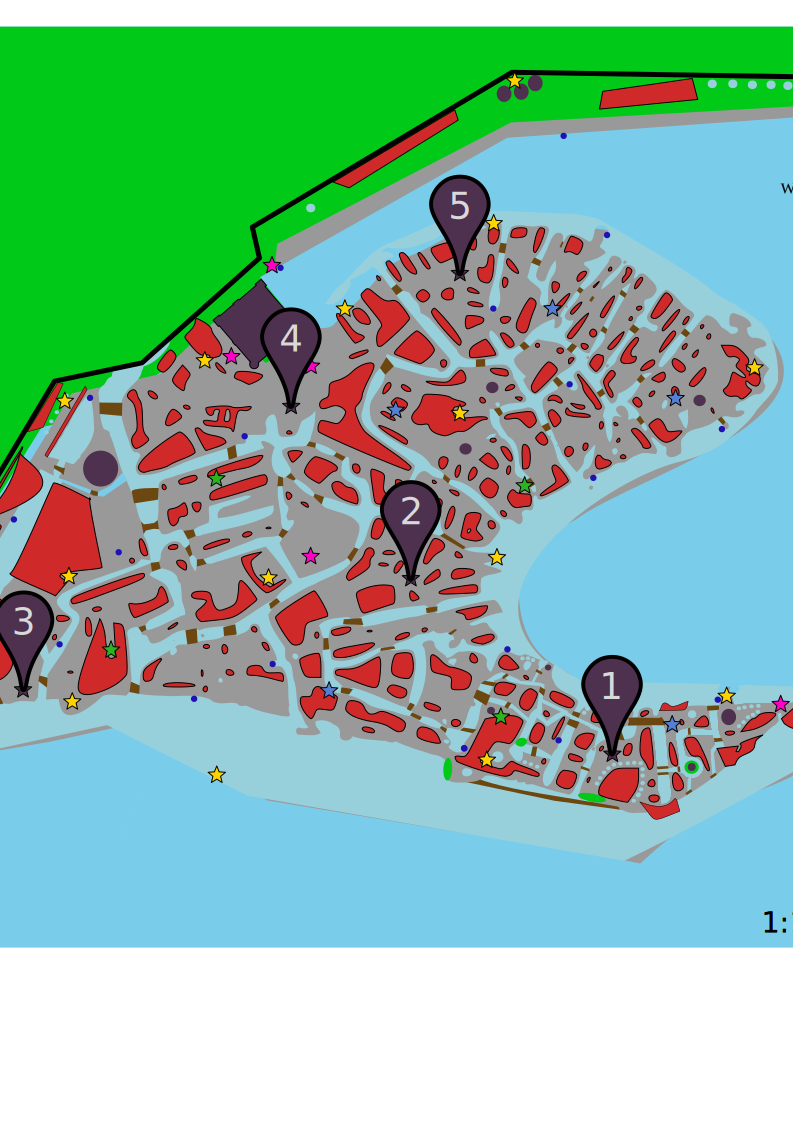
\includegraphics[width=\textwidth]{Images/Maps/dynamia}
  \caption{Map of Dynamia}
\end{figure}

The city is loosely based on Venice.

It is the capital of the Kingdom of Strangia. It is built on a lagoon and its streets are canals. Most of the quarters are placed on a small island connected to nearby ones by bridges.

It is a very beautiful and distinctive city, all the buildings are very colorful and there are many famous monuments. Thanks to its position, it is a very important business hub and there are merchants from many different countries. Despite the ongoing war, its market is very renowned and there you can find a lot of exotic products.

There are some guards and demons that patrol the city, but the atmosphere is quite peaceful. On direct orders of queen, each citizen has to do his best for the nation and any offender will be harshly punished.

There are some small shrubs that grow between the bricks of the building, quite big palms and vines on the walls. Some houses have beautiful and very manicured gardens, in particular in downtown.

On the streets there are some stray dogs and cats, mice and a lot of seagulls.

The city is divided in 4 macro areas and it has some characteristic landmarks that will be described here below.

For more reference images: \url{http://wastelandsteam.altervista.org/dynamia/}\\
Password: \textit{gld18}


\subsection{Macro areas}
\begin{figure}[H]
  \centering
  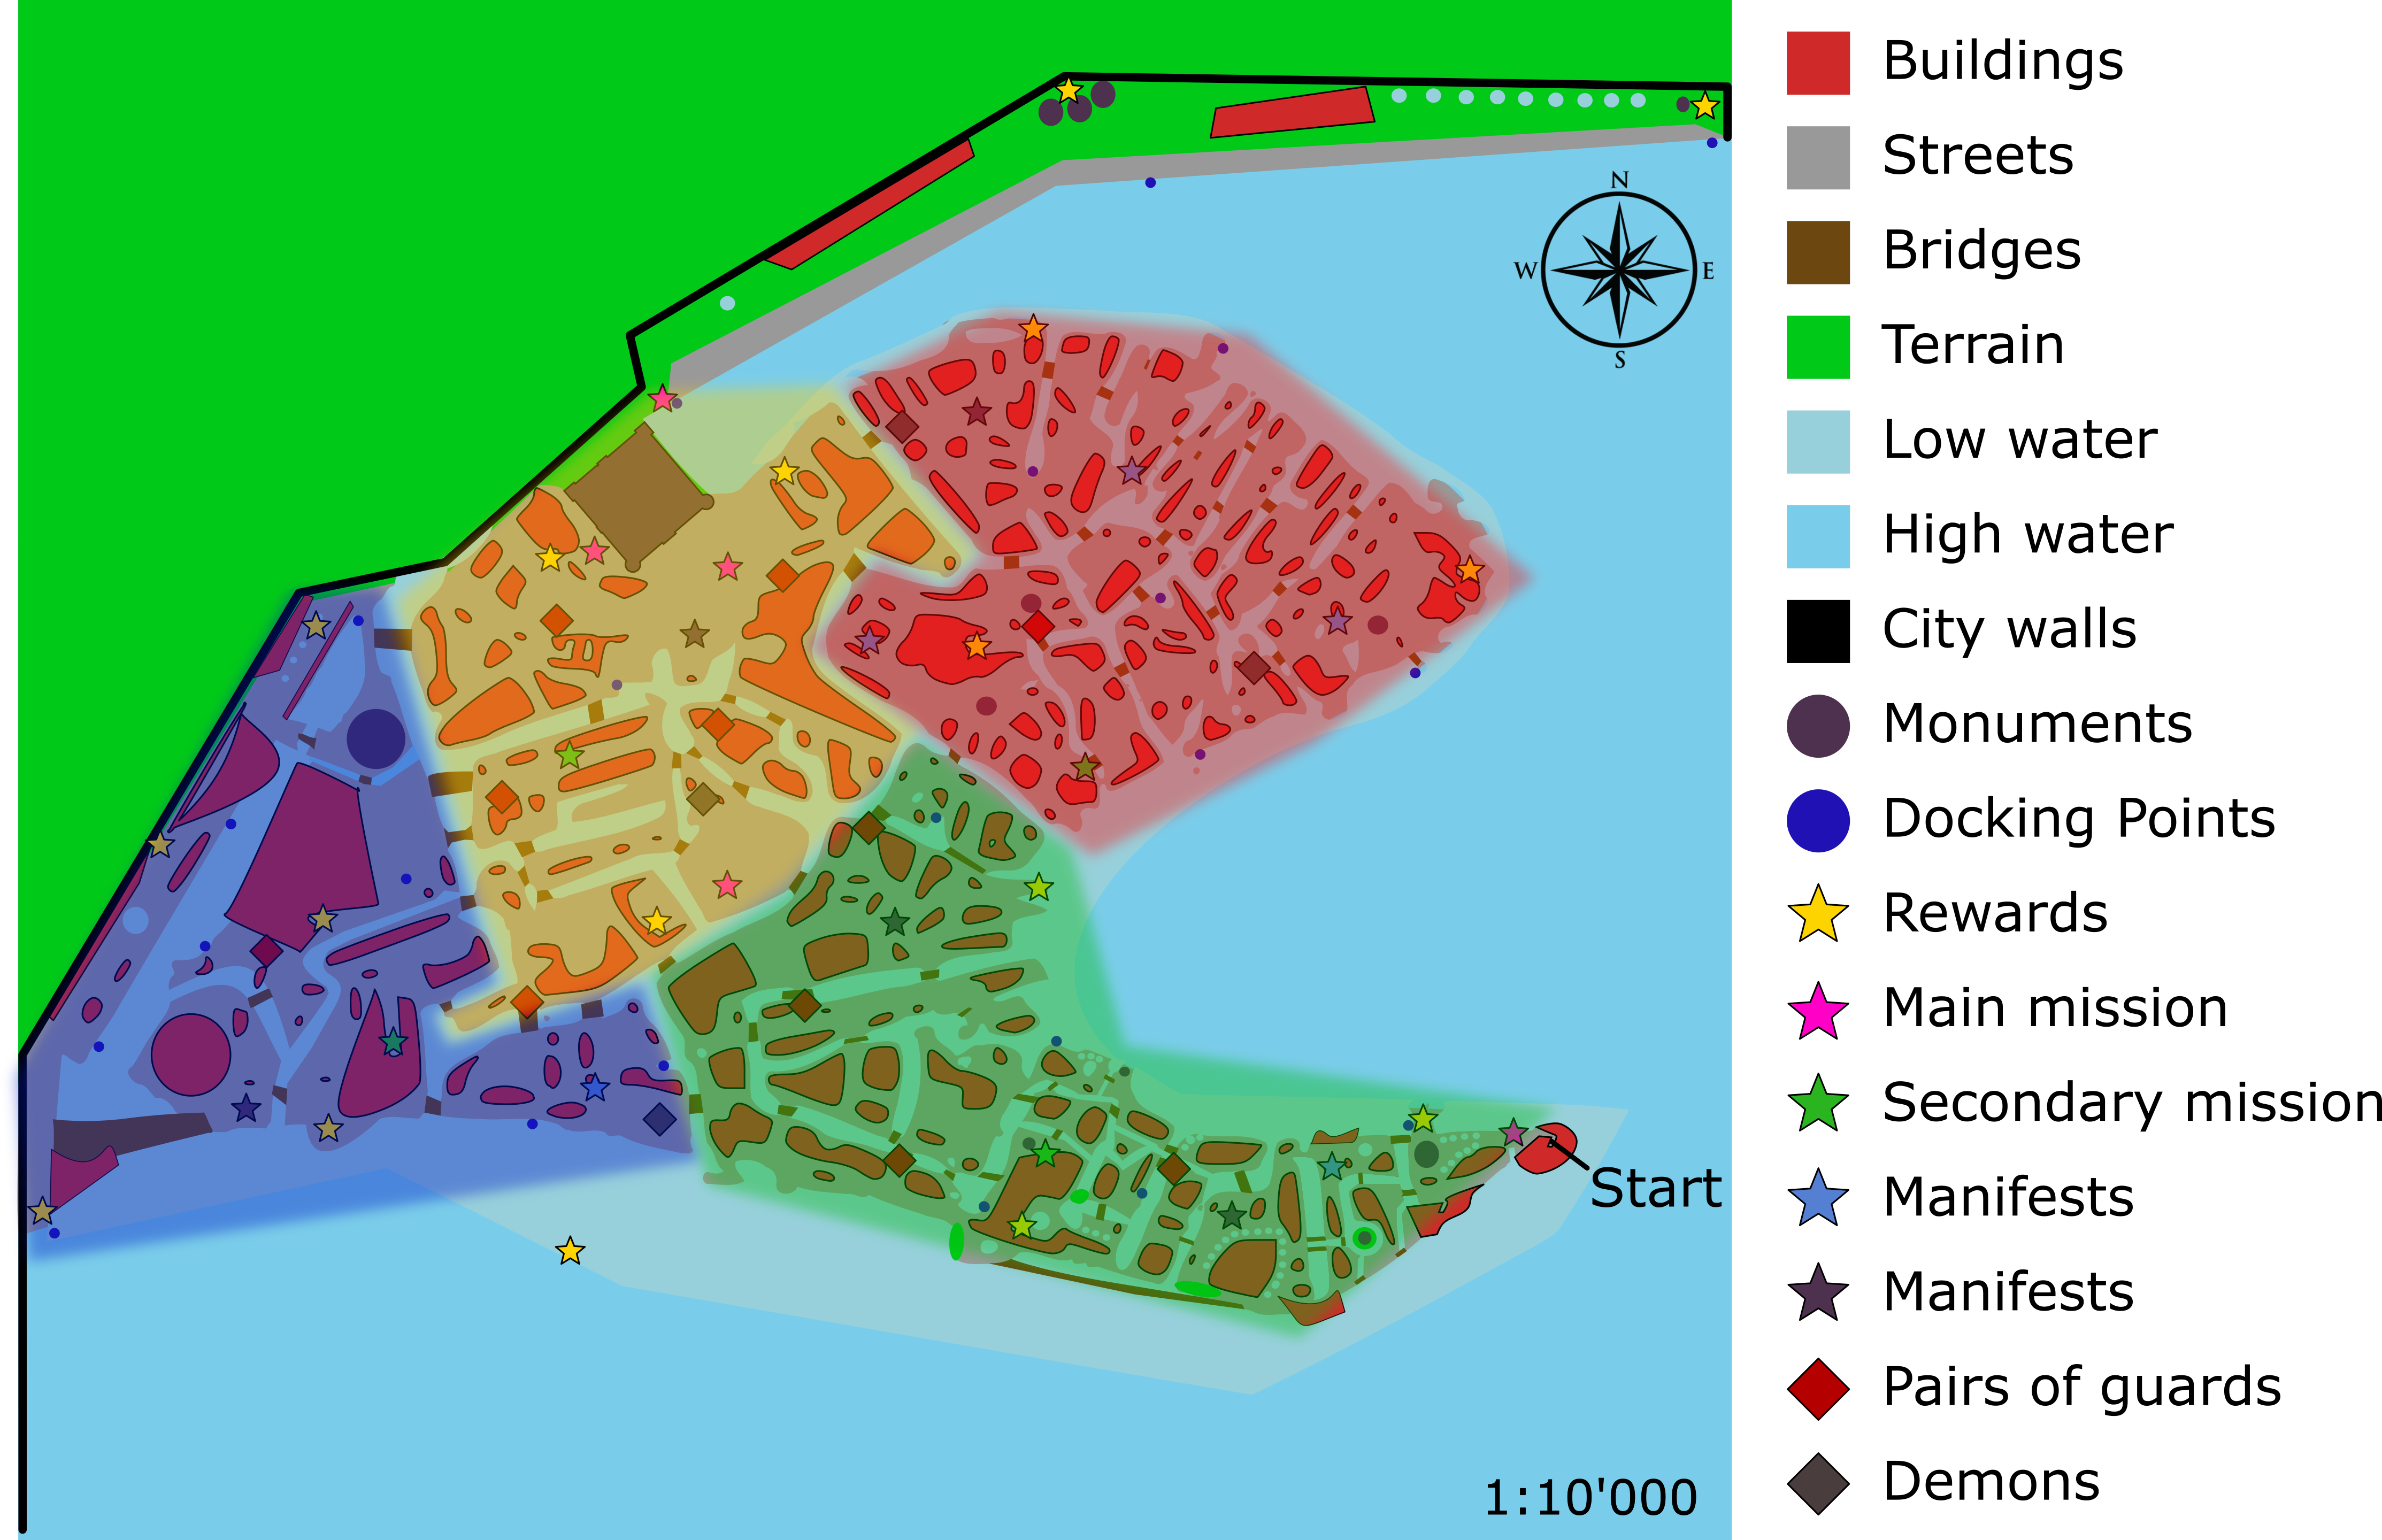
\includegraphics[width=\textwidth]{Images/Maps/dynamiaAreas}
  \caption{Macro areas of Dynamia}
\end{figure}

\subsubsection{Southern area (green)}
This is the first area that the player will see.

The southern area is the newest part of Dynamia. People who come from outside the city has chosen this area to build their house, in the outskirts of the city. Here it is common to see every kind of people from every part of the region and we can find a mix of cultures and languages. The high triumph arc in the end of the city can be seen from the sea and it is a "welcome" for all of the people who reach Dynamia.

\subsubsection{Central area (yellow)}
This is by far the richest area in the city. In fact here we can find the houses of  nobles and rich merchants as well as the castle and the market. Given this, here is common to find jewelries, merchants who sell luxury items and highly decorated villas on the canals.

In addition to the castle and the market that will be described in next paragraphs, another important landmark is the square in front of the castle itself. Here from early morning till evening, newsboys scream and shout trying to sell their newspapers to the people who pass by  or to simply announce the new rules and laws that the queen has issued.

\subsubsection{Harbor area (blue)}
The harbor occupies the western area of the city. On the large canal near the city walls we can a huge freight yard and some shipyards, the  other buildings in this zone are mostly houses of fishermen and and warehouses.

This area is the main door on the sea of the city and allows to big ships to enter into the city to drop off their supply or get repaired before heading to the open sea. Here we can find both the biggest bridge and the biggest monument of Dynamia. The bridge is a drawbridge that opens up to let cargo ships get in, while the monument represents the God of Fortune and here merchants and fishermen come to pray before they set sail.

\subsubsection{Ghetto area (gray)}
The ghetto area is called this way because, centuries before, it was the area where  minorities where confined. Nowadays it has changed and it is a working-class neighborhood where you can find people from all walks of life. Here life is cheaper than in the central area and so it is a good choice for travellers, poor people or people who can't afford something better, but even middle class people.

The streets are typically more crowded and dirtier; houses are not as elegant as in the center, generally built with only wood or concrete and without any sort of decoration.

We can find some little shops who sell fresh food and bread, some little factories and few handicraft workshop. So, differently from the scent of rare spices from the southern desert we can smell in the central area, here we can find only the smell of fish and smoke.


\subsection{Dead end}
\begin{figure}[H]
  \centering
  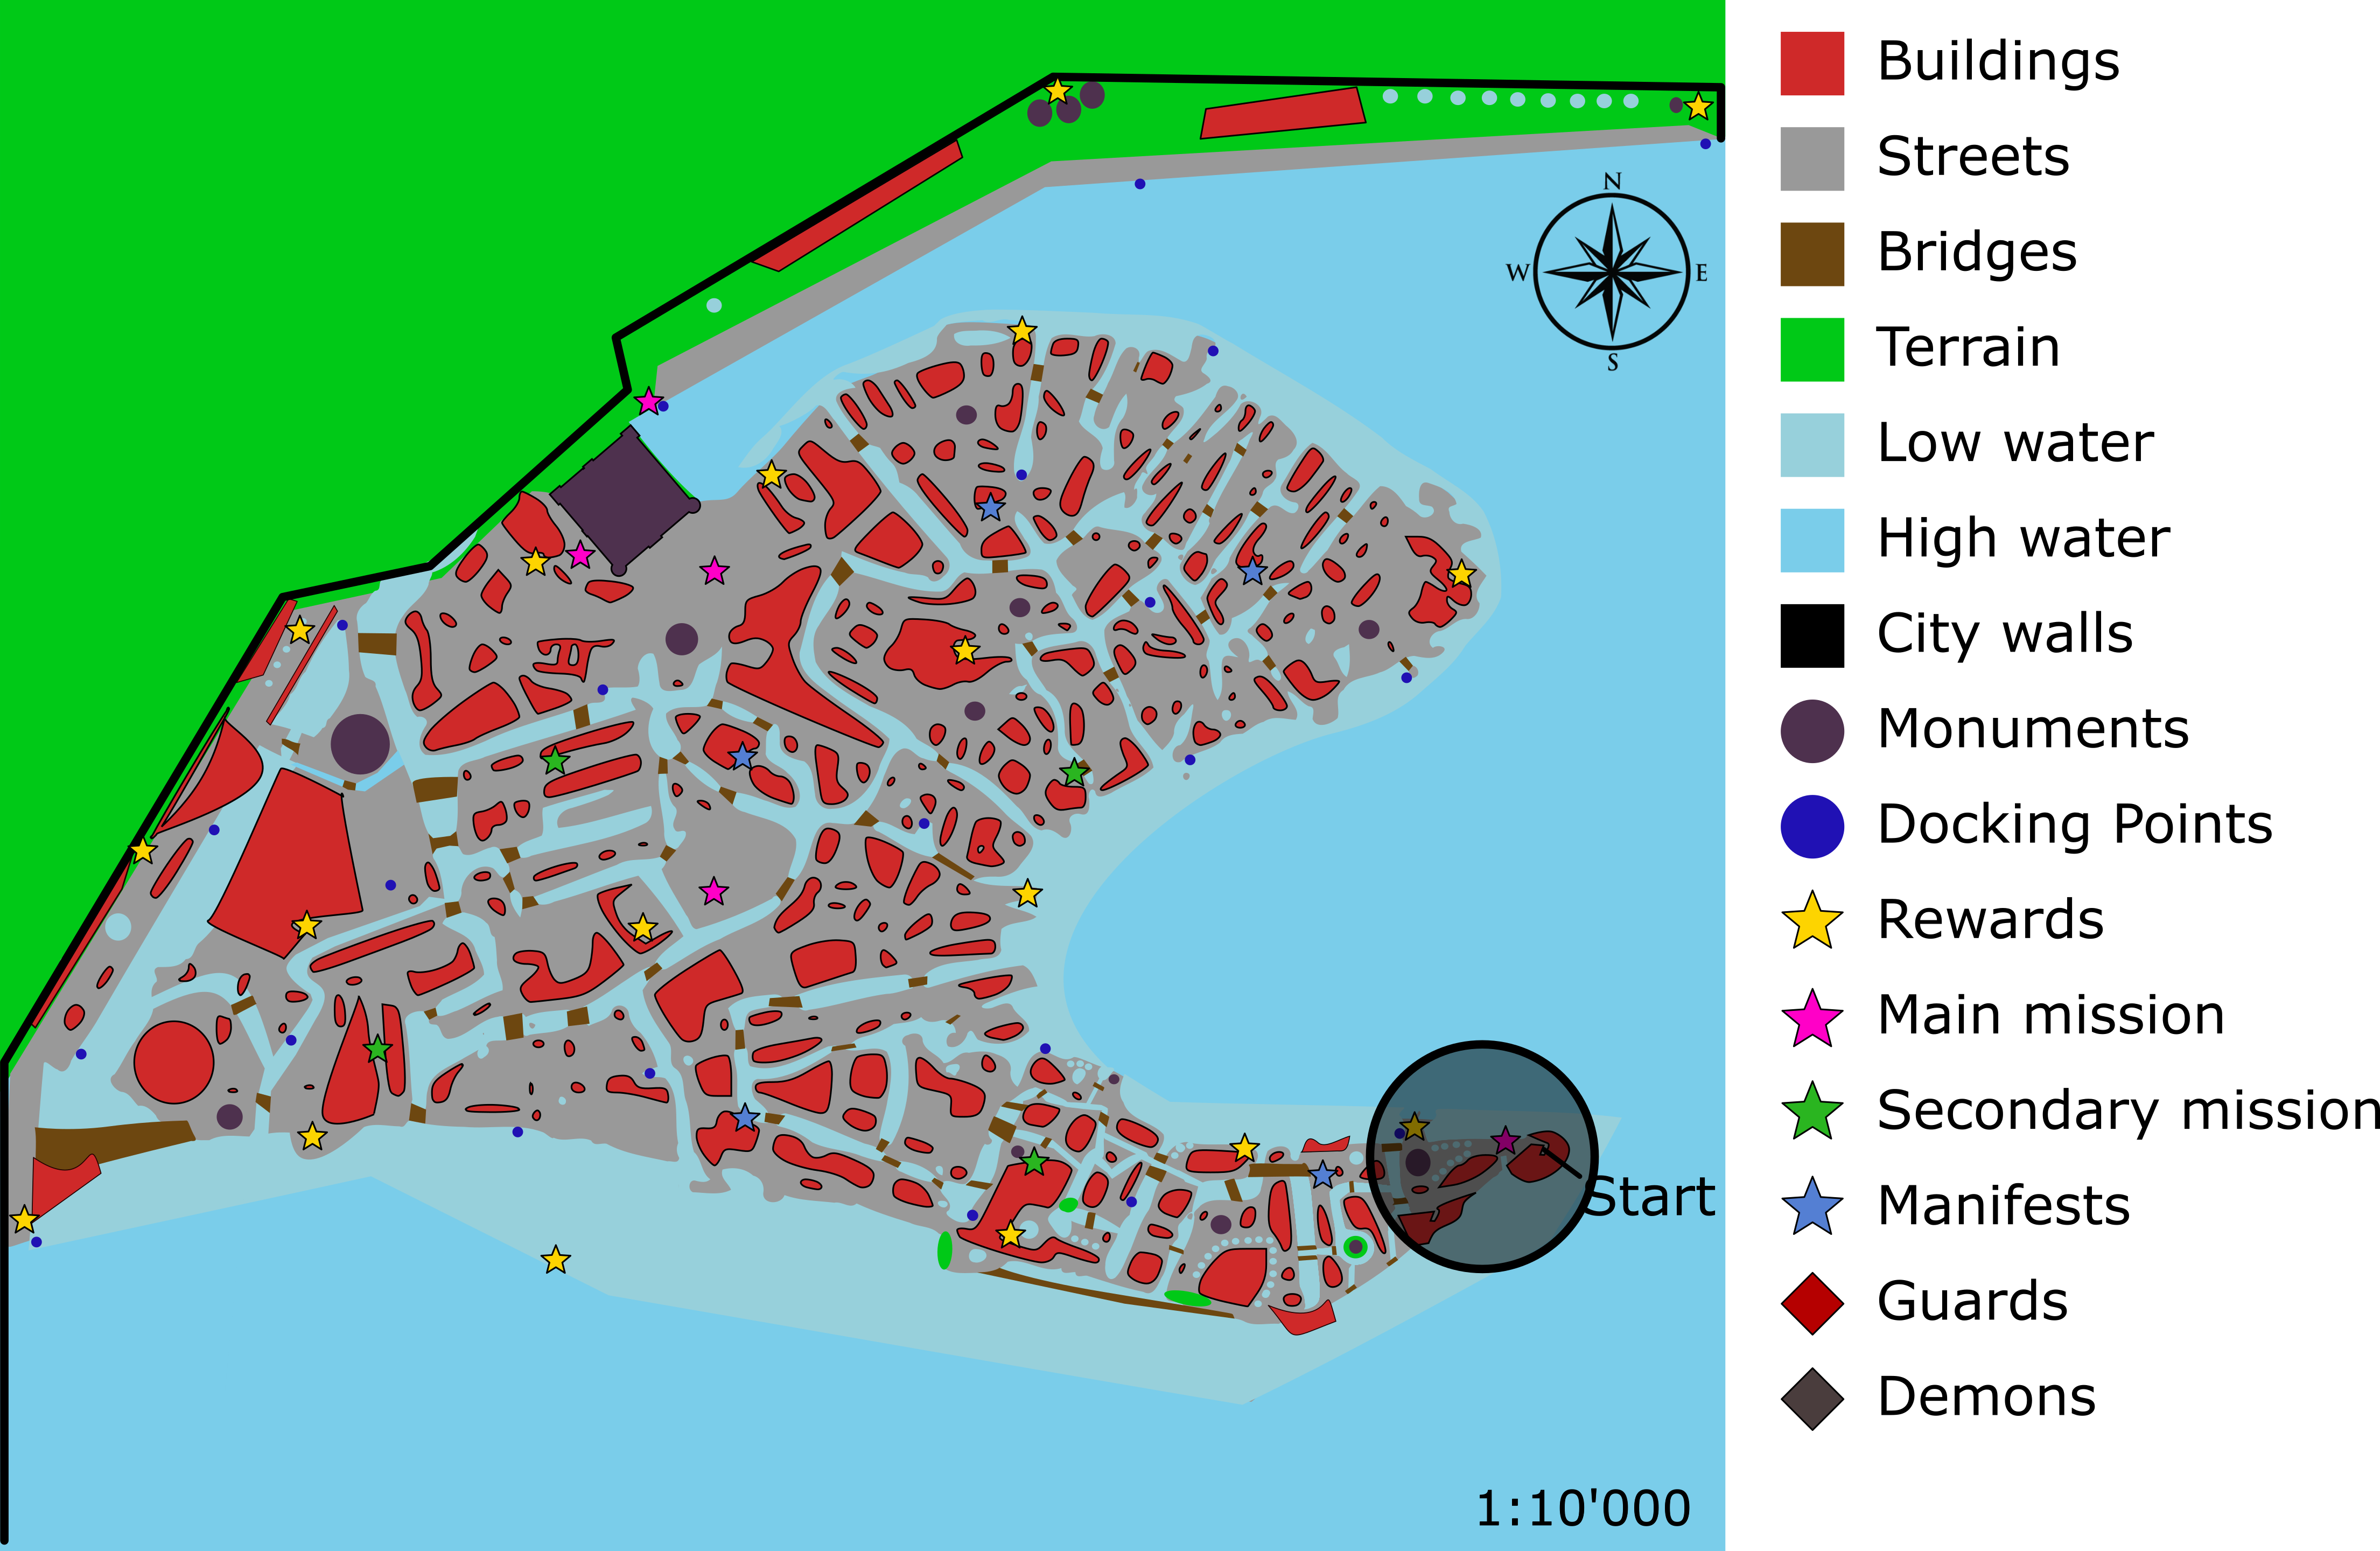
\includegraphics[width=\textwidth]{Images/Maps/dynamia_deadEnd}
  \caption{Dead end position}
\end{figure}

Dynamia ends here, in a neighborhood of colored houses that overlook on the canals. Some houses have sea view, instead, the others have their windows on a little, narrow, nice dead-end.

This short street connects the neighborhood to a big street leading to the central neighborhoods of Dynamia.

At the beginning of this boulevard there is a manifest and a panel with the map of the city.

The street is bordered by flowerbeds and fountains of every shape and it is loosely based on the \textit{Champs Elysees}.

From every point of the street you can see a big arc of triumph at the end of it that can be considered the entrance of Dynamia.

\begin{figure}[H]
  \centering
  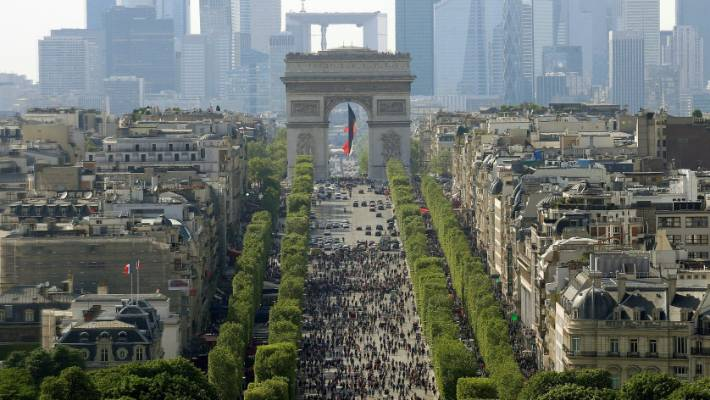
\includegraphics[width=8cm]{Images/Landmarks/arcOfTriumph}
  \caption{A references images of the arc of triumph}
\end{figure}

For more reference images: \url{http://wastelandsteam.altervista.org/dynamia/dead-end/}\\
Password: \textit{gld18}

\subsection{Market of Dynamia}
\begin{figure}[H]
  \centering
  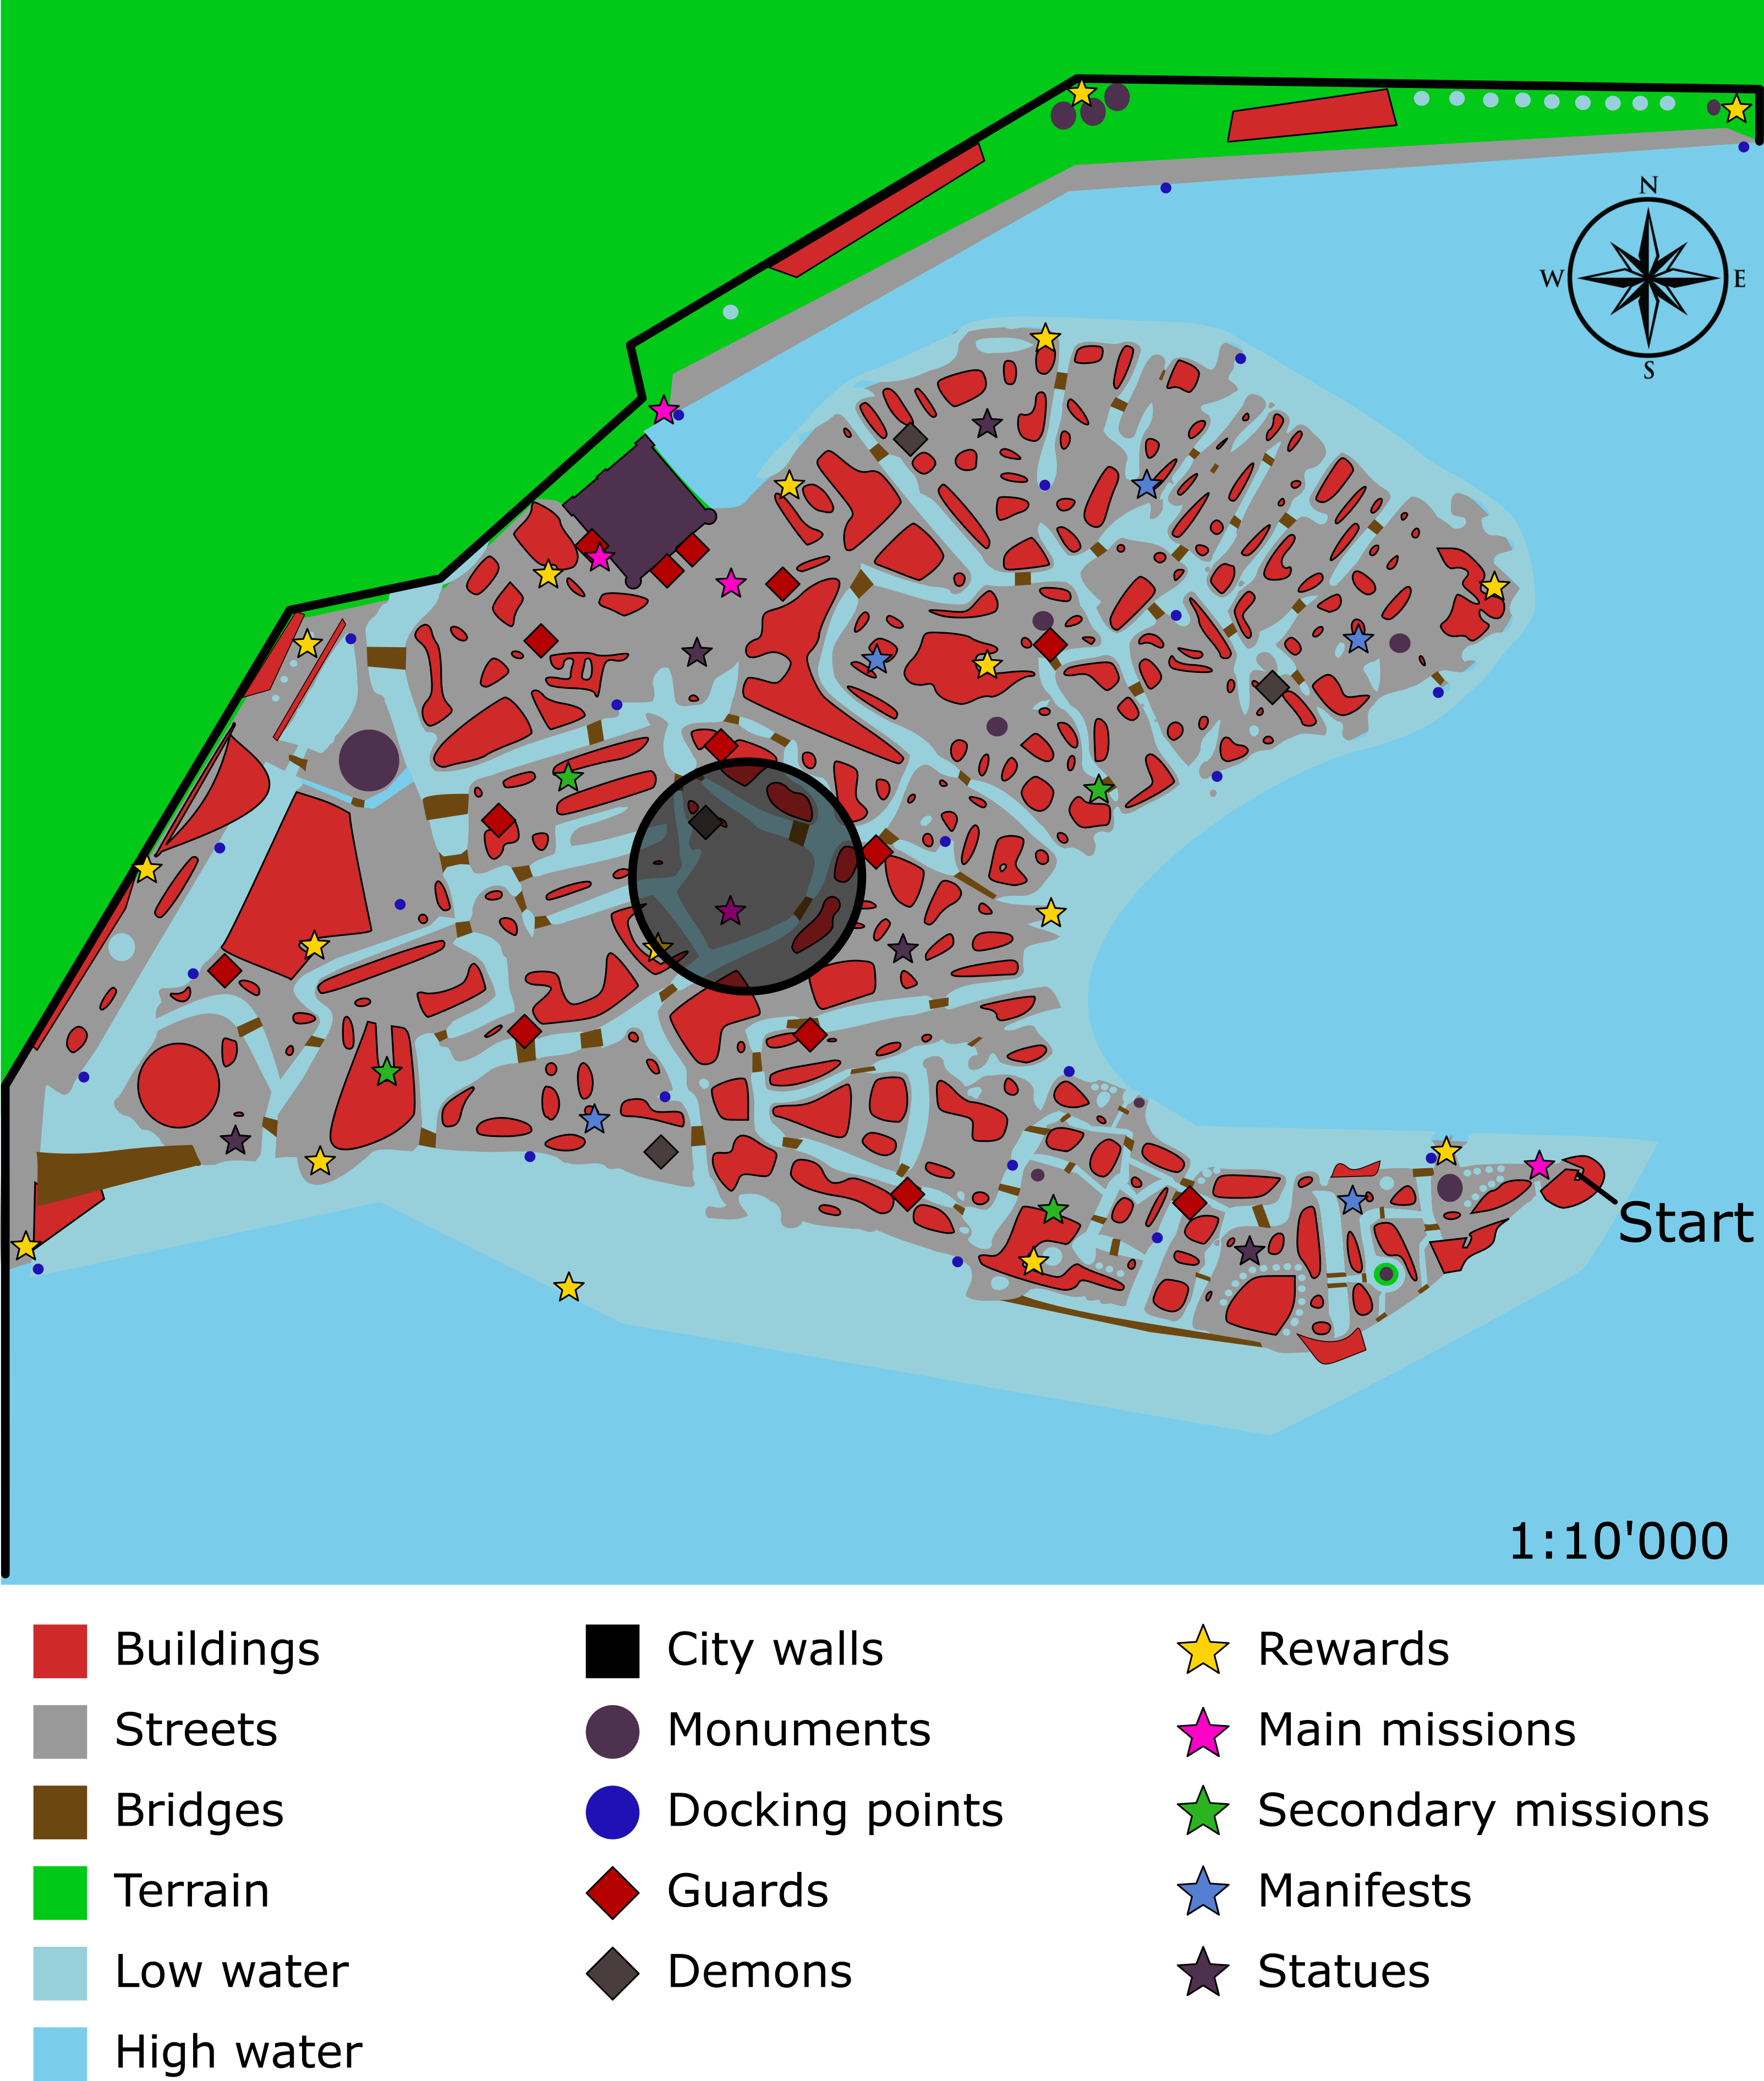
\includegraphics[width=\textwidth]{Images/Maps/dynamia_market}
  \caption{Market position}
\end{figure}

The Market is situated in a wide square positioned in the middle of the city. It is surrounded by many canals and it is the nerve centre of Dynamia where, everyday, people and merchants from every part of the region come to buy and sell any kind of merch. There are many stands that sell clothes, hats, wool and fabric and here the player could find some of the rarest materials to craft items.

The market is characterized by a constant buzz caused by the huge crowd that populates  the square during the daytime. During the late afternoon merchants and people start leaving the market and so it becomes a quiet place where Dynamians love to stay and walk in the evening.

In the south west corner the player will find the merchant that will help in finding a way to get inside the castle.
 
\begin{figure}[H]
  \centering
  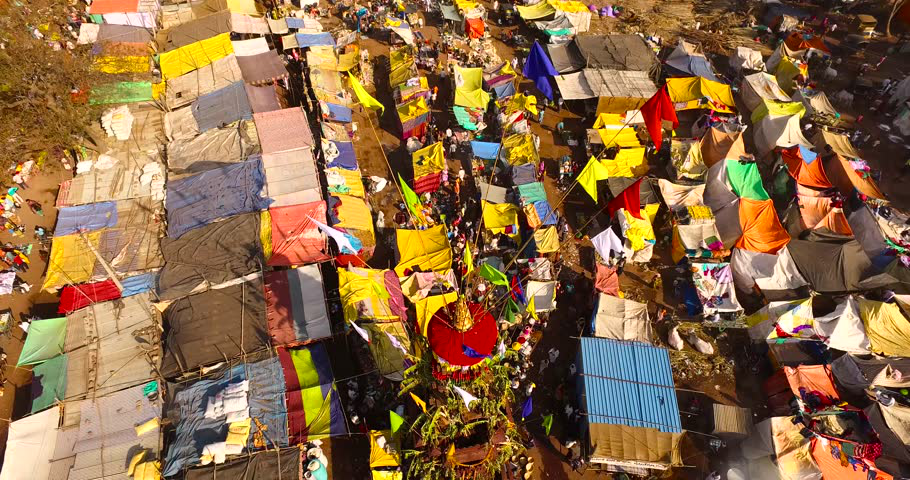
\includegraphics[width=\textwidth]{Images/Landmarks/market}
  \caption{Reference image for the market}
\end{figure}

For more reference images: \url{http://wastelandsteam.altervista.org/dynamia/market-of-dynamia/}\\
Password: \textit{gld18}

\subsection{Castle of Dynamia}
\begin{figure}[H]
  \centering
  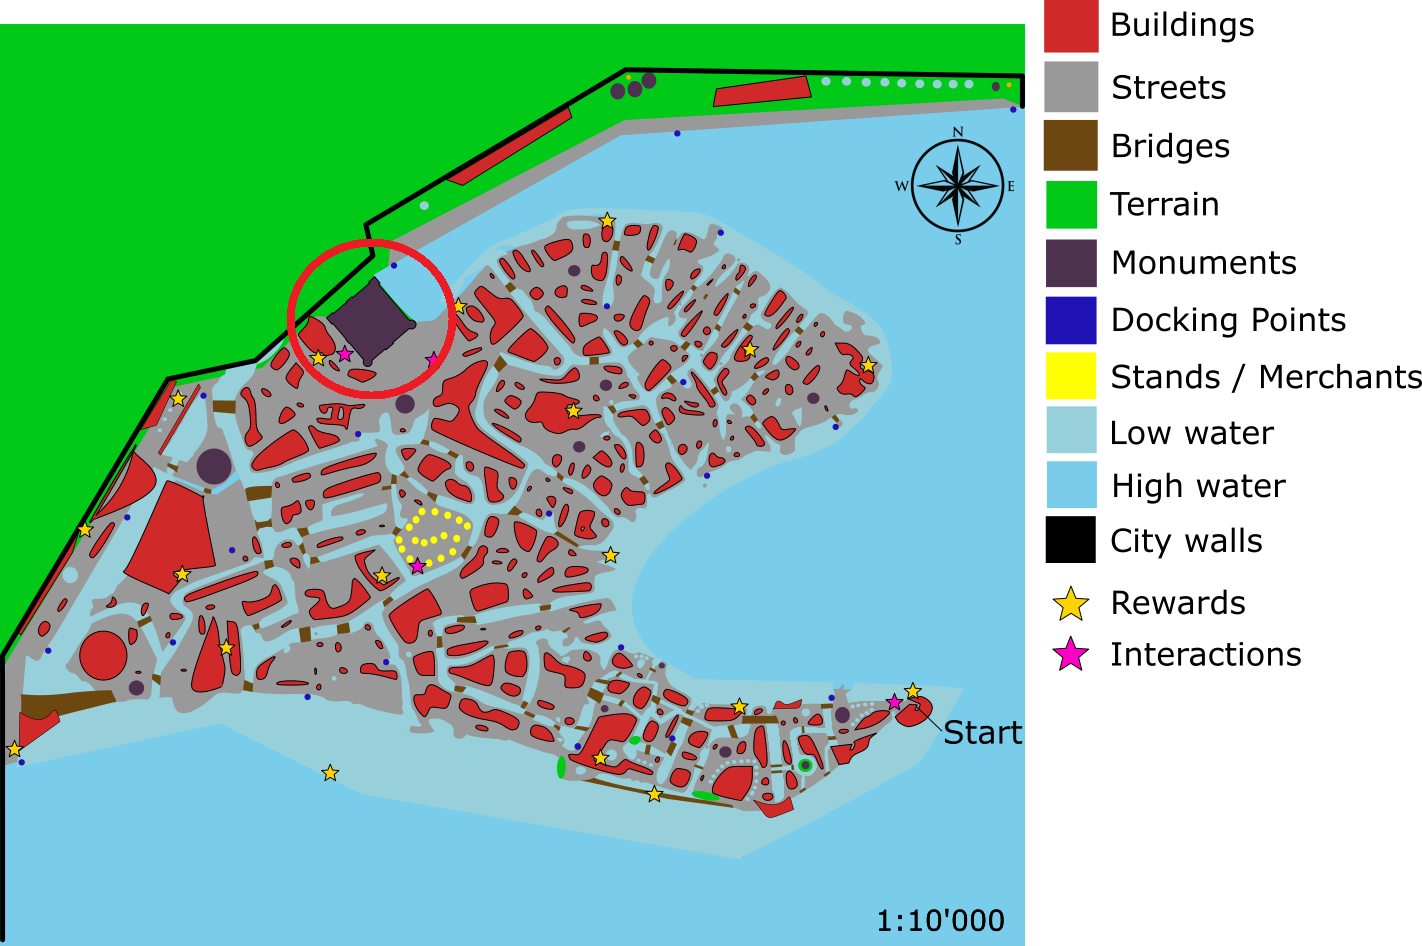
\includegraphics[width=\textwidth]{Images/Maps/dynamia_castleOfDynamia}
  \caption{Castle position}
\end{figure}

The castle of Dynamia is loosely based on the Sforza Castle of Milan.

It is placed upon a rocky promontory and it is the main entrance to Dynamia from the continent. It has been designed by the court magician of Dynamia centuries ago, and it has many secret passages. The player can access some of this secret passages by solving puzzles.

It is made of stones, it has a big courtyard and two buildings: one on the west, heavily fortified, and one, more refined, on the north for the royal family. Mizar lives in the northern building, but the player can visit only the main courtyard and a portion of the western area.

There are human guards and demons that patrol the castle. They are ordered to arrest any intruder. The most powerful enemy is the captain of the guards.

\begin{figure}[H]
  \centering
  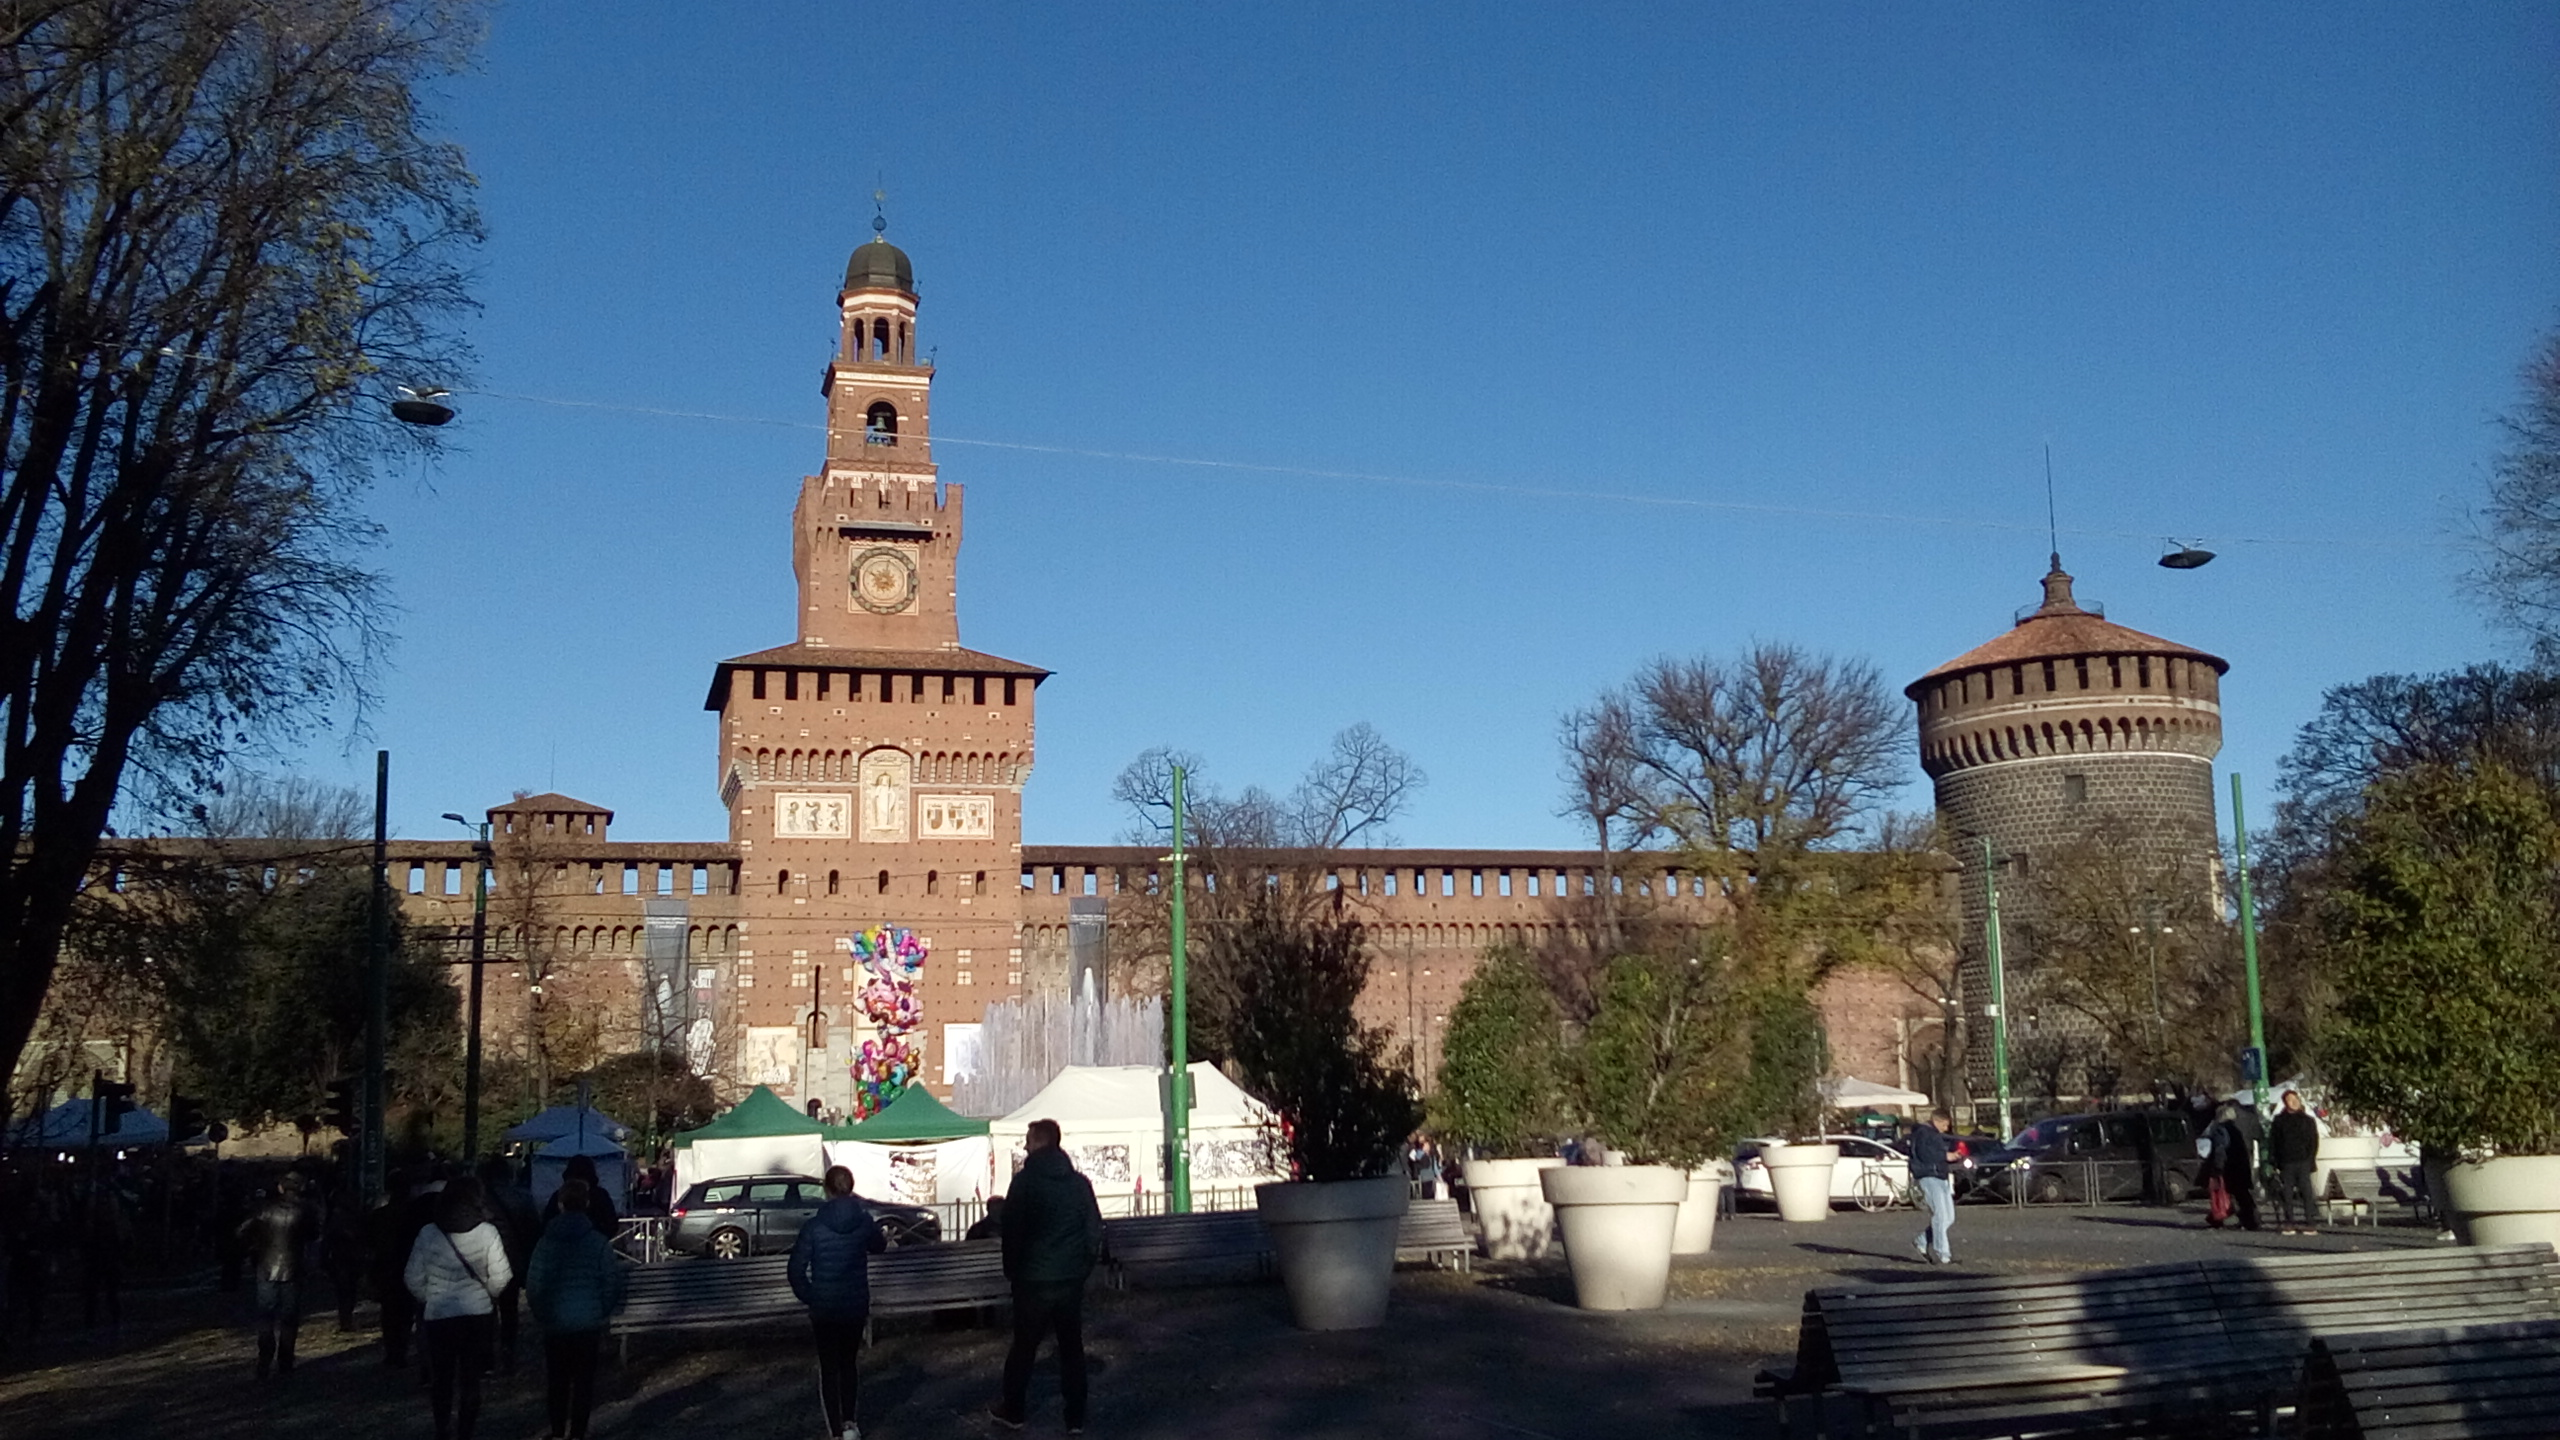
\includegraphics[width=\textwidth]{../../../References/Images/Dynamia/CastleOfDynamia/20181208_100357}
  \caption{Reference image for the Castle of Dynamia}
\end{figure}

\begin{figure}[H]
  \centering
  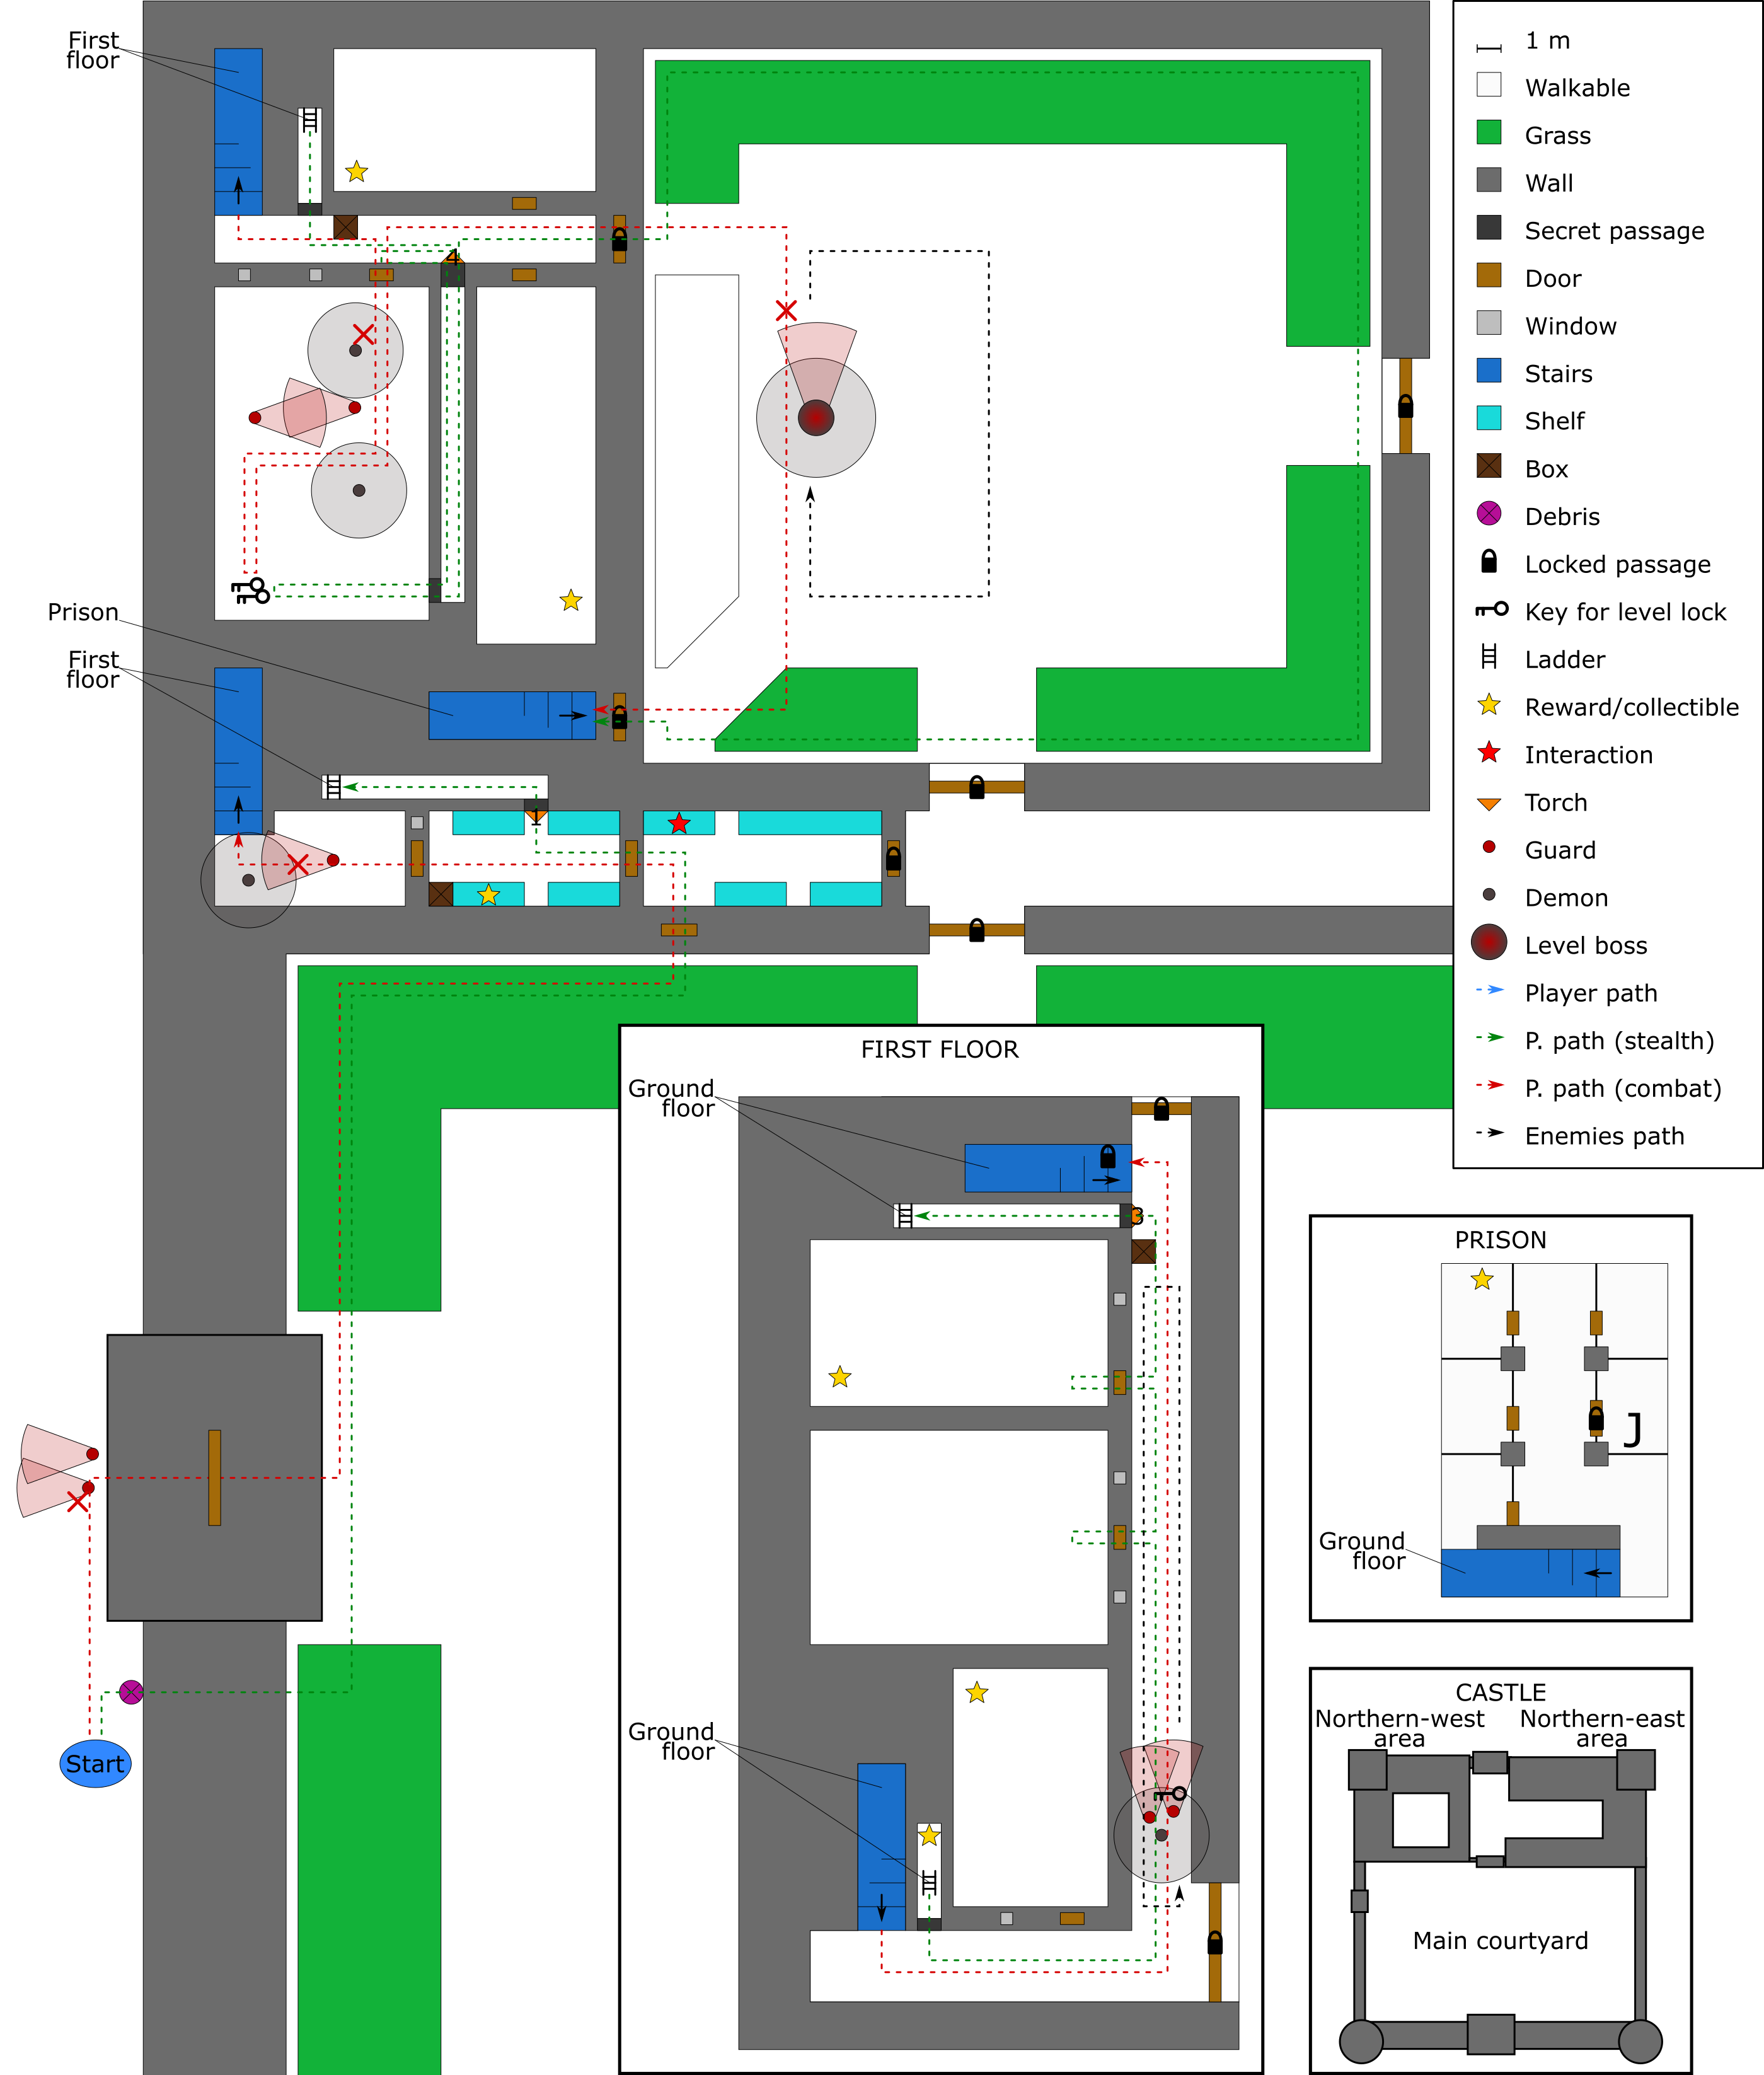
\includegraphics[width=\textwidth]{Images/Maps/castleOfDynamia}
  \caption{Map of the Castle of Dynamia}
\end{figure}

For more reference images: \url{http://wastelandsteam.altervista.org/dynamia/castle-of-dynamia/}\\
Password: \textit{gld18}

\subsubsection{Docking point}
\begin{figure}[H]
  \centering
  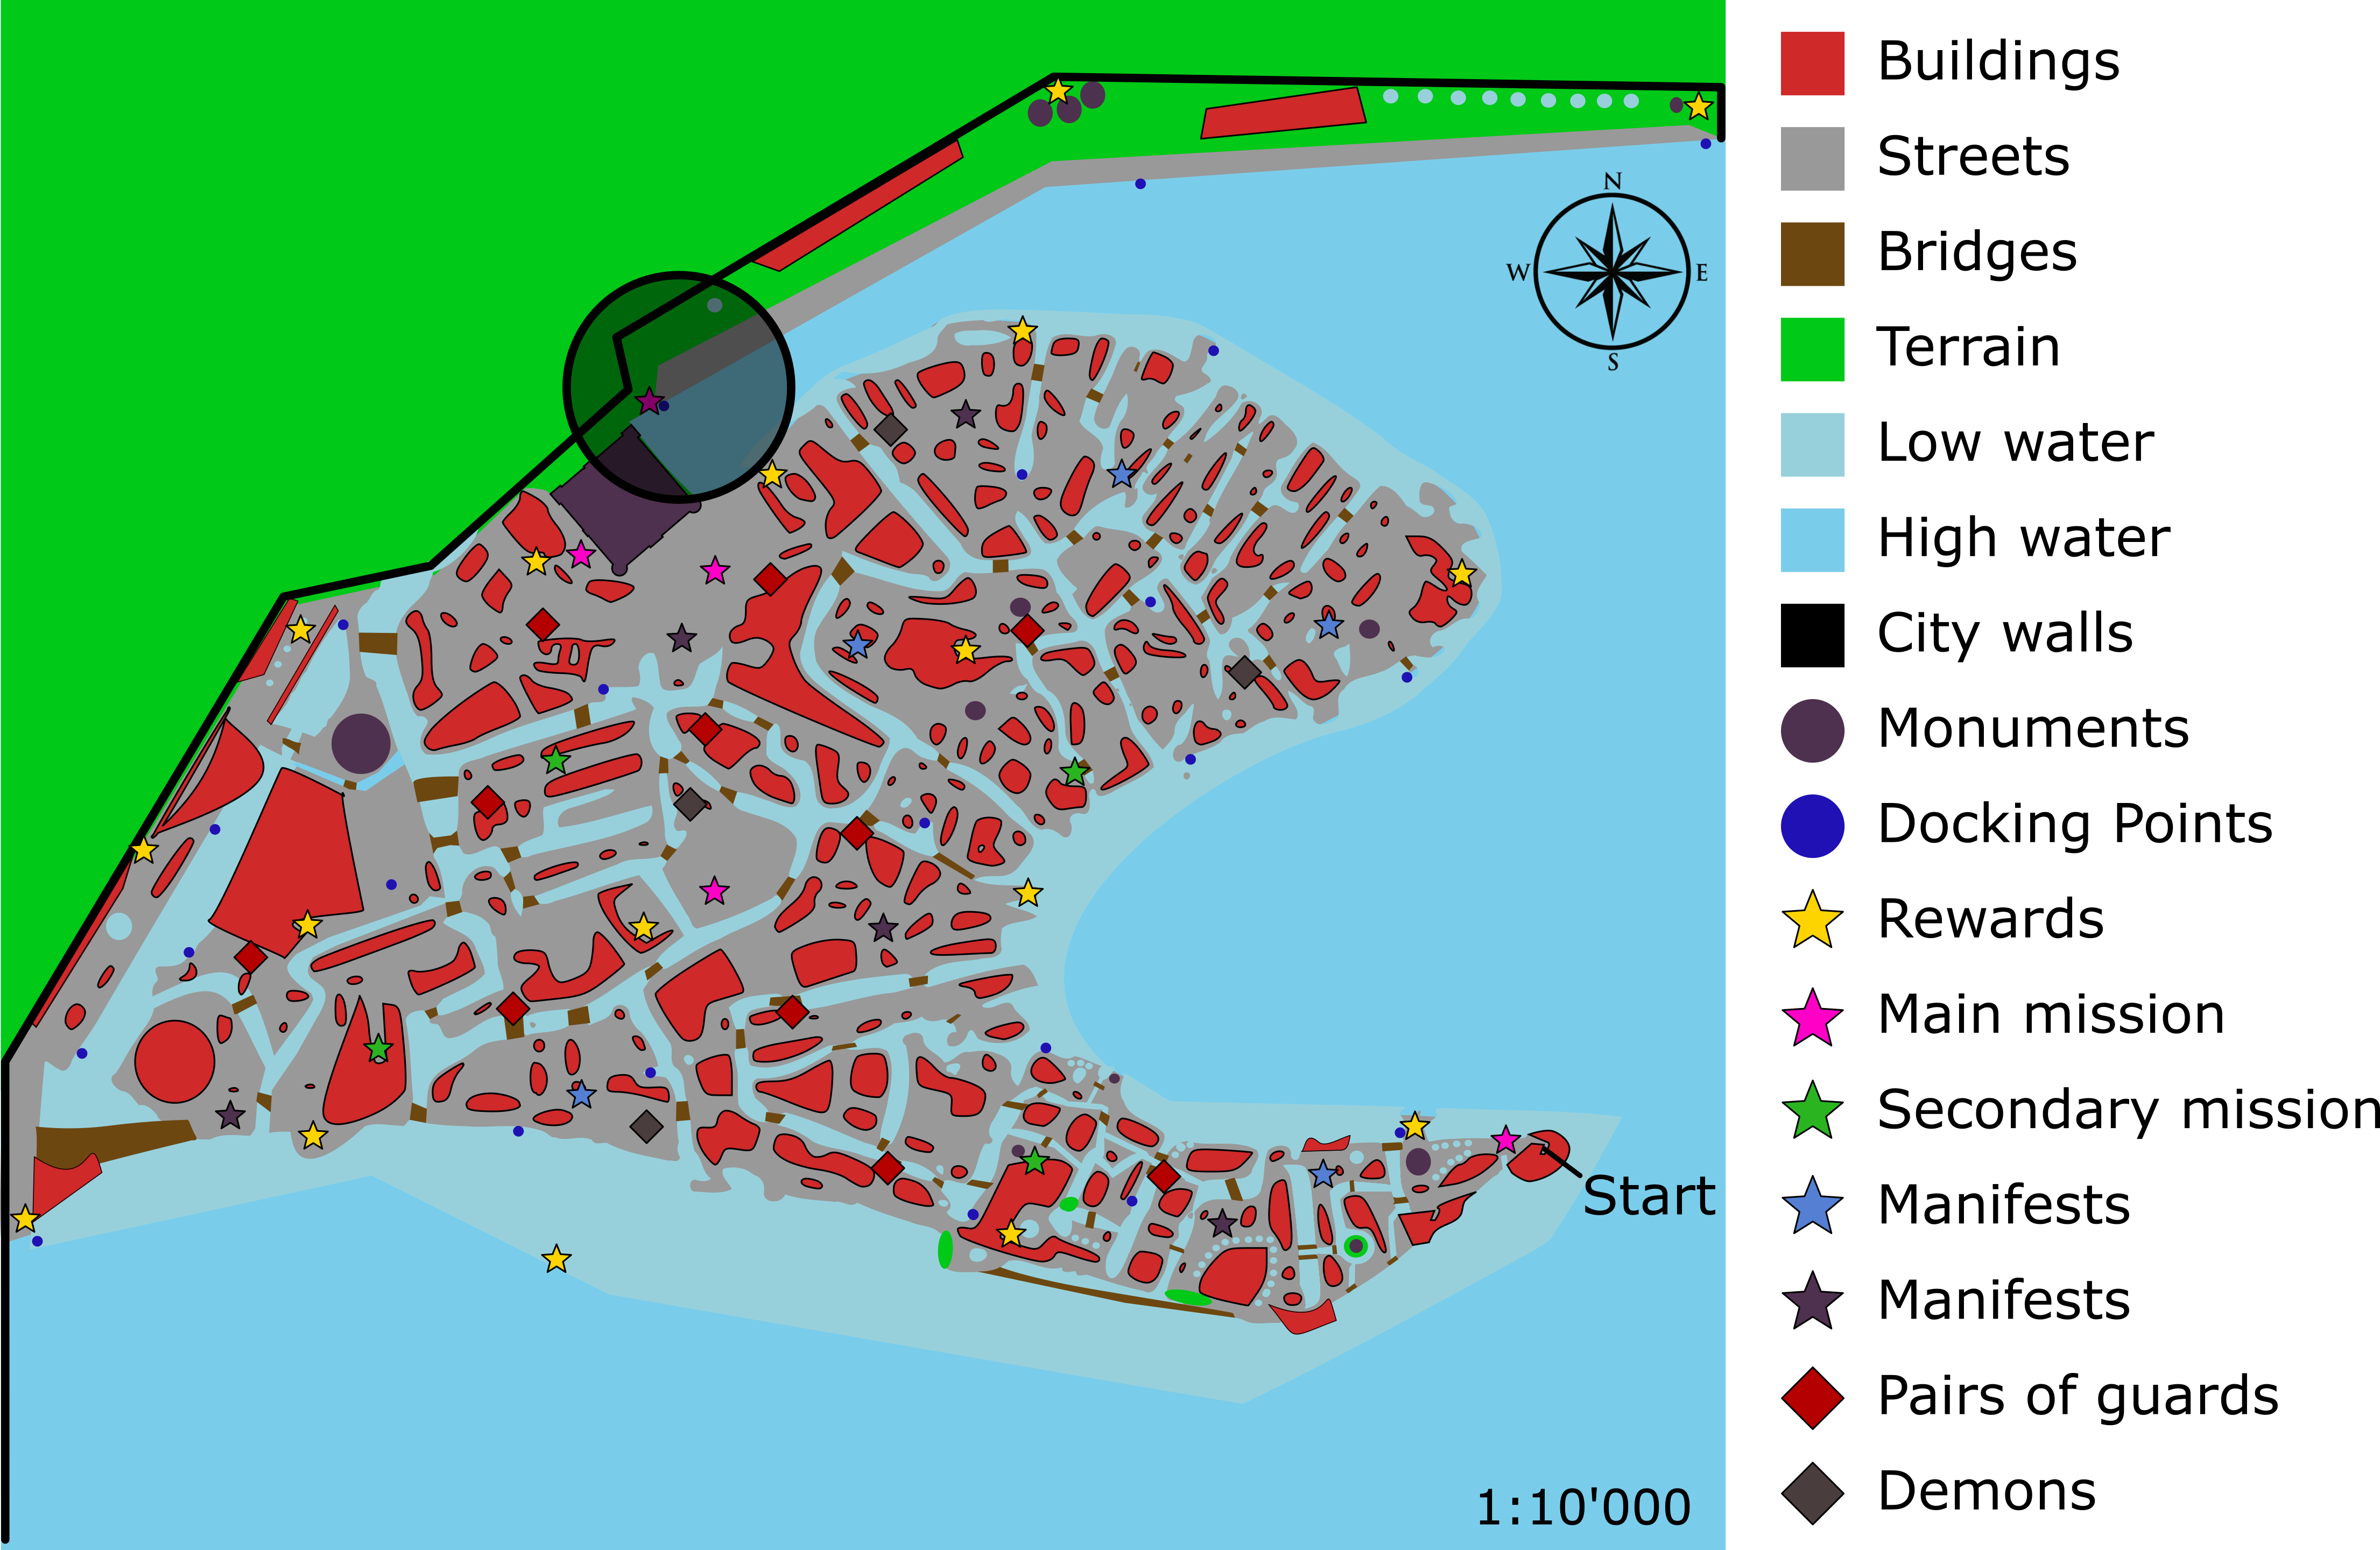
\includegraphics[width=12cm]{Images/Maps/dynamia_dockingPoint}
  \caption{Docking point position}
\end{figure}
  
In this area we may find wooden poles placed in the water, decorated with flowers, where gondoliers and fishers tie their little boats and gondolas, and  stone stairs that lead to small platforms on the canals.

In the center of the area there is a small street and a fountain which has in its middle a statue representing Mizar, surrounded by flowers. Mizar keeps her right arm up holding her scepter that spills water.

Behind the docking point the player can see the gigantic city walls that defend Dynamia from enemy attacks.

\begin{figure}[H]
  \centering
  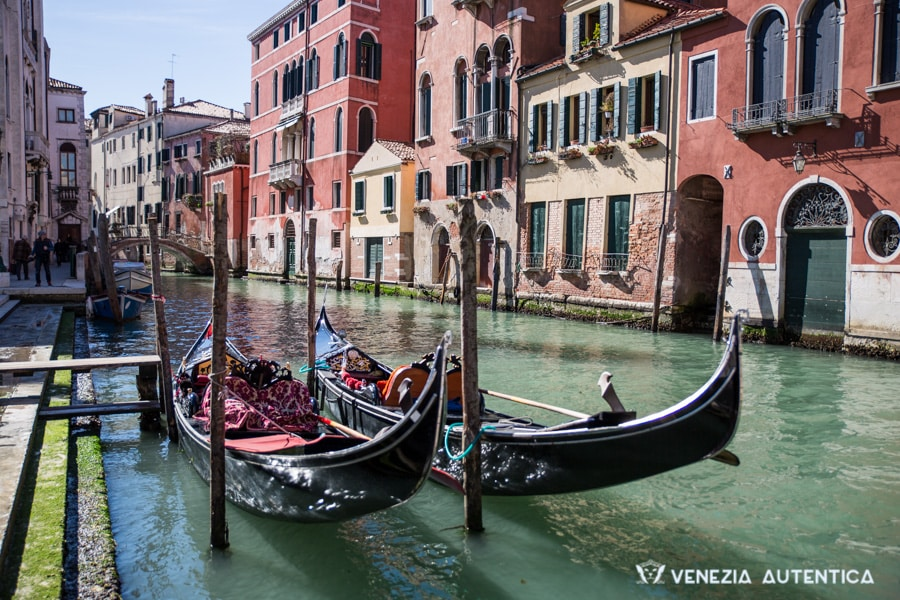
\includegraphics[width=\textwidth]{Images/Landmarks/dockingPoint}
  \caption{References image for the docking point}
\end{figure}
For more reference images: \url{http://wastelandsteam.altervista.org/dynamia/docking-point/}\\
Password: \textit{gld18}
